\section{OGC}
\label{sec:ogc}

Alle hiervoor beschreven informatie gaat over bestaande technieken waarop verder gewerkt wordt. Vanaf nu gaat het meer over het geospatiale. Dit zijn technieken die gerespecteerd en toegepast moeten worden om zo het uiteindelijke onderzoek te kunnen doen. 

OGC staat voor Open Geospatial Consortium. Dit is een wereldwijde community die zich inzet voor het verbeteren van de manier hoe omgegaan wordt met geospatiale locatie informatie. Het OGC maakt standaarden om geospatiale informatie beschikbaar te stellen, zodat deze door gebruikers op een optimale en zo uniform mogelijke manier bereikt kan worden \cite{ogcdocs}.

Het OGC voorziet vele standaarden, daarom zullen enkel de relevante besproken worden.

\subsection{WKT}
WKT staat voor \textit{Well-known text}. Dit is een opmaak taal voor het representeren van geometrie objecten op een map. Hierbij worden de coordinaten van een positie gescheiden door een spatie (eerst de x coördinaat, daarna de y coördinaat), opeenvolgende posities binnen één structuur worden gescheiden door een komma \cite{ogcdocs}. 

De primitieve geometrieën zijn ``\textit{Point}'', ``\textit{LineString}'' en ``\textit{Polygon}''. Een ``\textit{Point}'' staat voor één exacte locatie op een map. Een ``\textit{LineString}'' gaat dan weer over een lijn, dit zijn dus de verbindingen tussen verschillende punten (bijvoorbeeld van punt1 naar punt2 en van punt2 naar punt3). Ten slotte is er een ``\textit{Polygon}'', wat staat voor een vlak. Hierbij heeft het OGC nog enkele andere voorwaarden opgesteld. Een ``\textit{Polygon}'' moet topologisch gesloten zijn, wat betekent dat het laatste punt hetzelfde moet zijn als het eerste. Daar bovenop kan een ``\textit{Polygon}'' bestaan uit een buitenste en binnenste lineaire ring. De buitenste ring slaat op het vlak, terwijl de binnenste ring slaat op een vlak dat uit het grotere vlak gehaald wordt. Hierbij stelt het OGC dat de locaties van de buitenste ring in tegenwijzerszin gegeven moeten zijn, terwijl deze van de binnenste ring in wijzerszin moeten zijn \cite{ogcdocs}.

Een verduidelijking van primitieve geometrieën is te zien in \tableref{tab:wkt_primitives}. Hierin is het eerste punt van een figuur steeds opgevuld voor verduidelijking. Bij een ``\textit{Polygon}'' met twee ringen wordt ook direct duidelijk waarom de dubbele haken er staan.

\begin{table}[ht]
\centering
\begin{tabular}{ |l|c|p{8cm}| } 
 \hline
 \rowcolor{TableHeaderColor} Type & \multicolumn{2}{c|}{Example} \\ \hline
 
 \rowcolor{TableColor} \multirow{4.5}{*}{Point} & \raisebox{-\height+2mm}[0pt][20mm]{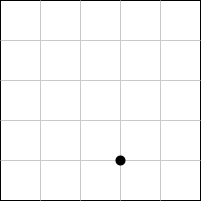
\includegraphics[width=20mm, height=20mm]{images/wkt_point.png}} & POINT (30 10) \\ \hline
 
 \rowcolor{TableColor} \multirow{4.5}{*}{LineString} & \raisebox{-\height+2mm}[0pt][20mm]{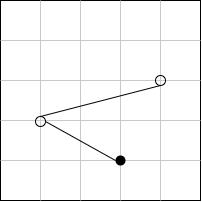
\includegraphics[width=20mm, height=20mm]{images/wkt_line.png}} & LINESTRING (30 10, 10 20, 40 30) \\ \hline
 
 \rowcolor{TableColor} & \raisebox{-\height+2mm}[0pt][20mm]{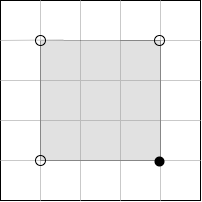
\includegraphics[width=20mm, height=20mm]{images/wkt_polygon1.png}} & POLYGON ((40 10, 40 40, 10 40, 10 10, 40 10)) \\ \cline{2-3}
 
 \rowcolor{TableColor} \multirow{-2}{*}{Polygon} & \raisebox{-\height+2mm}[0pt][20mm]{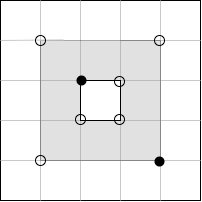
\includegraphics[width=20mm, height=20mm]{images/wkt_polygon2.png}} & POLYGON ((40 10, 40 40, 10 40, 10 10, 40 10), (20 30, 30 30, 30 20, 20 20, 20 30) \\ \hline
\end{tabular}
\caption{Primitieve geometrieën.}
\label{tab:wkt_primitives}
\end{table}

Naast de primitieve geometrieën zijn er ook de meerdelige geometrieën. Hierin bestaan ``\textit{MultiPoint}'', ``\textit{MultiLineString}'' en ``\textit{MultiPolygon}''. Deze staan respectievelijk voor één of meer van de overeenkomstige primitieve geometrieën. Ter verduidelijking van de meerdelige geometrieën is er ook een klein voorbeeld voorzien in \tableref{tab:wkt_multipart}. Hierbij gelden uiteraard dezelfde conventies als bij de primitieve geometrieën.


\begin{table}[ht]
\centering
\begin{tabular}{ |l|c|p{8cm}| } 
 \hline
 \rowcolor{TableHeaderColor} Type & \multicolumn{2}{c|}{Example} \\ \hline
 
 \rowcolor{TableColor} \multirow{4.5}{*}{MultiPoint} & \raisebox{-\height+2mm}[0pt][20mm]{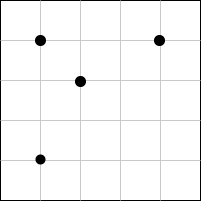
\includegraphics[width=20mm, height=20mm]{images/wkt_multipoint.png}} & MULTIPOINT ((10 40), (10 10), (20 30), (40 40)) \\ \hline
 
 \rowcolor{TableColor} \multirow{4.5}{*}{MultiLineString} & \raisebox{-\height+2mm}[0pt][20mm]{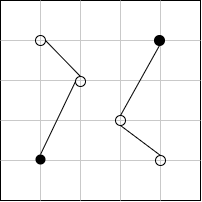
\includegraphics[width=20mm, height=20mm]{images/wkt_multiline.png}} & MULTILINESTRING ((10 10, 20 30, 10 40), (40 40, 30 20, 40 10)) \\ \hline
 
 \rowcolor{TableColor} & \raisebox{-\height+2mm}[0pt][20mm]{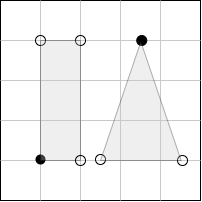
\includegraphics[width=20mm, height=20mm]{images/wkt_multipolygon1.png}} & MULTIPOLYGON (((10 10, 20 10, 20 40, 10 40, 10 10)), ((35 40, 25 10, 45 10, 35 40))) \\ \cline{2-3}
 
 \rowcolor{TableColor} \multirow{-2}{*}{MultiPolygon} & \raisebox{-\height+2mm}[0pt][20mm]{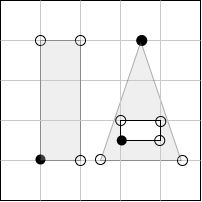
\includegraphics[width=20mm, height=20mm]{images/wkt_multipolygon2.png}} & MULTIPOLYGON (((10 10, 20 10, 20 40, 10 40, 10 10)), ((35 40, 25 10, 45 10, 35 40), (30 15, 30 20, 40 20, 40 15, 30 15))) \\ \hline
\end{tabular}
\caption{Meerdelige geometrieën.}
\label{tab:wkt_multipart}
\end{table}

\subsection{GML}
GML staat voor \textit{Geography Markup Language}. GML is een XML gramair die gedefinieerd is door het OGC met als doel om geospatiale informatie uit te drukken. GML doet dus hetzelfde als WKT, maar met andere notaties. Het is wel opmerkelijk dat het bij GML enkel mogelijk is om primitieve geometrieën te beschrijven, dus geen meerdelige geometrieën. Aangezien deze standaard minder vaak gebruikt wordt, zal deze ook minder gedetailleerd besproken worden. Zo zijn er drie verschillende manieren om coördinaten weer te geven in GML \cite{ogcdocs}:
\begin{itemize}
    \item ``<gml:coordinates>'': bij deze \textit{tag} worden de coördinaten gescheiden door een komma. Indien er meerdere locaties na elkaar komen worden deze dan weer gescheiden door een spatie.
    \item ``<gml:pos>'': bij deze \textit{tag} worden de coördinaten gescheiden door een spatie. Hier is het niet mogelijk om meerdere locaties na elkaar te laten komen.
    \item ``<gml:posList>'': deze \textit{tag} is gelijkaardig aan de ``pos'' \textit{tag}, maar hier is het wel mogelijk om meerdere locaties na elkaar te laten komen. Deze worden dan opnieuw gescheiden door een spatie.
\end{itemize}

Een kort voorbeeld van de ``posList'' notatie is te zien in \listingref{listing:gml}. Hierin wordt het voorbeeld van ``\textit{LineString}'' uit \tableref{tab:wkt_primitives} herschreven naar de GML notatie. Hierbij van het ``srsDimension'' attribuut op. Dit geeft aan hoeveel dimensies het punt heeft.

\begin{listing}[ht]
\begin{minted}{xml}
<gml:LineString gml:id="p21"
    srsName="http://www.opengis.net/def/crs/EPSG/0/4326">
    <gml:posList srsDimension="2">30 10 10 20 40 30</gml:posList>
</gml:LineString >
\end{minted}
\caption{Voorbeeld GML bij LineString.}
\label{listing:gml}
\end{listing}

\subsection{GeoSPARQL}
Ook GeoSPARQL is een standaard van het OGC. GeoSPARQL is gemaakt voor het representeren en queryen van geospatiale data op het semantische web. Zo definieerd GeoSPARQL een vocabulair voor het representeren van geospatiale gegevens in RDF. Verder is het belangrijk te weten dat GeoSPARQL een uitbreiding is op de SPARQL query taal, met als doel het verwerken van geospatiale gegevens. GeoSPARQL is gemaakt om zowel systemen die gebaseerd zijn op kwalitatieve spatiale redenering als systemen die gebaseerd zijn op kwantitatieve spatiale berekeningen te huisvesten. Kortom zal GeoSPARQL nieuwe filter functies definiëren voor \gls{gisdef} (\acrshort{gis}) queries, gebruik makend van standaarden die gedefinieerd zijn door het OGC. Dit is echter een zeer korte en beperkte uitleg over GeoSPARQL, de gedetailleerde specificatie worden toegelicht in \sectionref{sec:geosparql}.